\documentclass[12pt, oneside]{article}
\usepackage[letterpaper, margin=1in]{geometry}
\usepackage[english]{babel}
\usepackage[utf8]{inputenc}
\usepackage{amsmath}
\usepackage{amsfonts}
\usepackage{amssymb}
\usepackage{tikz}
\usepackage{tkz-fct}

\usepackage{fancyhdr}
\pagestyle{fancy}
\fancyhf{}
\rhead{\thepage \\Name: \hspace{1.5in}.\\}
\lhead{BECA / Dr. Huson / 11.2 Algebra 2 \\* 31 May 2018 \\* \textbf{Pretest: Study packet}}

\vspace{1cm}

\renewcommand{\headrulewidth}{0pt}

\title{Problem set template}
\author{Chris Huson}
\date{May 2018}

\begin{document}
%\maketitle

\subsubsection*{\\* \textnormal{Answer in pen. Show work. Graph carefully using pencil.}}

\begin{enumerate}

\item Write $\sqrt[3]x \cdot \sqrt{x}$ as a single term with a rational exponent. %Alg2 Regents Jun2017
\\*[1.5in]

\item Explain how $\displaystyle \left(3^{\frac{1}{5}} \right)^2$ can be written as the equivalent radical expression $\sqrt[5]9$. \\[1.5in]%Alg2 Regents Aug2016


\item Given $i$ is the imaginary unit, $(2-yi)^2$ in simplest form is what? \\[1.5in]%Alg2 Regents Jun2016

\item What is the expression $6xi^3(-4xi+5)$ is equivalent to?  %Alg2 Regents Jun2017 multiple choice


\newpage
\item Sketch a graph of a cubic polynomial with the following characteristics: 
\begin{itemize}
\item three negative, real zeros
\item as $x \rightarrow + \infty$, $f(x) \rightarrow + \infty$
\item as $x \rightarrow - \infty$, $f(x) \rightarrow - \infty$
\end{itemize}
\begin{center}
    \begin{tikzpicture}[scale=2/4]
    \draw[thick,<->] (-7.5,0) -- (7.5,0) node[anchor=north west] {\textbf{x}};
    \draw[thick,<->] (0,-7.5) -- (0,7.5) node[anchor=south east] {\textbf{y}};
    \end{tikzpicture}
\end{center} %Alg2 Regents Jun2016 MC

\item Given: $f(x)=x^2+ x - 2$ and $g(x)=x-1$\\*[5pt]
Express $2 \bullet g(x) - f(x)$ as a polynomial in standard form. \\[3in] %Alg2 Regents Jan2018

\newpage
\item Find algebraically the zeros for  $g(x)=x^3-2x^2-5x+6$.\\*[2in]
On the set of axes below, graph $y=g(x)$.
\begin{center}
    
\begin{tikzpicture}[scale=2.54/4]
    \draw[step=1cm,gray,very thin] (-10,-10) grid (10,10);
    \draw[thick,<->] (-10.5,0) -- (10.5,0) node[anchor=north west] {\textbf{x}};
    \draw[thick,<->] (0,-10.5) -- (0,10.5) node[anchor=south east] {\textbf{y}};
    %\foreach \x in {-6, -4, -2, 2, 4, 6} \draw (\x cm,1pt) -- (\x cm,-1pt) node[anchor=north] {$\x$};
    %\foreach \y in {5} \draw (1pt,\y cm) -- (-1pt,\y cm) node[anchor=east] {50};
    %\foreach \y in {-5} \draw (1pt,\y cm) -- (-1pt,\y cm) node[anchor=east] {-50};    \tkzInit[xmin=-5,xmax=5,ymin=-7,ymax=7,ystep=1]
%    \tkzFct[color=black,thick,<->,domain = -3.4:7] {0.1*(x*x-4)*(x-5)};
    \end{tikzpicture}
\end{center} %Alg2 Regents Aug2016

\newpage 

\item On the grid below, sketch a cubic polynomial whose zeros are 1, 3, and $-2$.\\*
\begin{center}
    
\begin{tikzpicture}
    \draw[step=0.25in,gray,very thin] (0,0) grid (12.7,12.7);
    \end{tikzpicture}
\end{center} %Alg2 Regents Jan2018


\newpage
\item Given $f(x)=3x^2+7x-20$ and $g(x)=x-2$, state the quotient and remainder of $\displaystyle \frac{f(x)}{g(x)}$, in the form $\displaystyle q(x)+ \frac{r(x)}{g(x)}$. \\[4in] %Alg2 Regents Jan2017

\item Determine if $x-5$ is a factor of $2x^3-4x^2-7x-10$. Explain your answer. %Jun2016 Regents FR

\newpage

\item The function below models the average price of gas in a small town since January 1st.
\[G(t)=-0.0049t^4 + 0.0923t^3 - 0.56t^2 +1.166t+3.23 \text{, where } 0 \leq t \leq 10.\]
If $G(t)$ is the average price of gas in dollars and $t$ represents the number of months since January 1st, the absolute maximum $G(t)$ reaches over the given domain is about what value, to the nearest cent? \\[3in]%Alg2 Regents Jan2018

\item A rabbit population doubles every 4 weeks. There are currently five rabbits in a restricted area. If $t$ represents the time, in weeks, and $P(t)$ is the population of rabbits with respect to time, about how many rabbits will there be in 98 days? %Alg2 Regents Jan2017 

\newpage

\item Researchers in a local area found that the population of rabbits with an initial population of 20 grew continuously at the rate of 5\% per month. The fox population had an initial value of 30 and grew continuously at the rate of 3\% per month.\\*[5pt]
Find, to the \emph{nearest tenth of a month}, how long it takes for these populations to be equal. \\[3in] %Alg2 Regents Jan2018

\item In New York State, the minimum wage has grown exponentially. In 1966, the minimum wage was \$1.25 an hour and in 2015, it was \$8.75. Algebraically determine the rate of growth to the \emph{nearest percent}.

\newpage

\item Jim is looking to buy a vacation home for \$172,600 near his favorite southern beach. The formula to compute a mortgage payment, $M$, is $\displaystyle M=P \cdot \frac{r(1+r)^N}{(1+r)^N-1}$ where $P$ is the principal amount of the loan, $r$ is the monthly interest rate, and $N$ is the number of monthly payments. Jim’s bank offers a monthly interest rate of 0.305\% for a 15-year mortgage.\\*[5pt]
With no down payment, determine Jim’s mortgage payment, rounded to the nearest dollar.\\*[3in]
Algebraically determine and state the down payment, rounded to the \emph{nearest dollar}, that Jim needs to make in order for his mortgage payment to be \$1100.
 %Alg2 Regents Jun2017 multiple choice


\newpage

\item Graph $y=400(.85)^{2x}-6$ on the set of axes below.
\begin{center}
    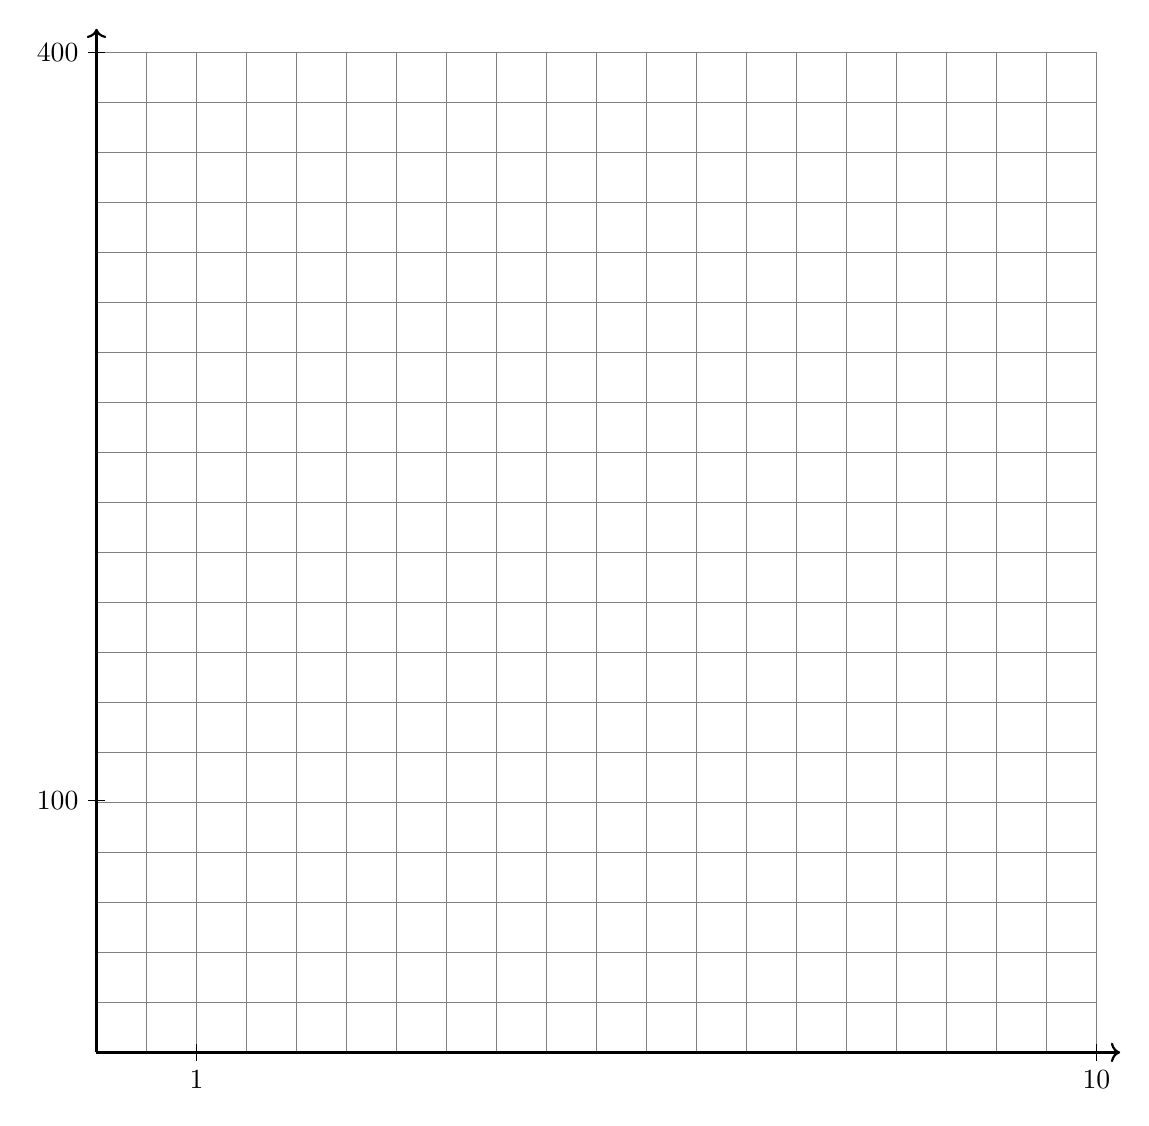
\begin{tikzpicture}
    \draw[step=0.25in,gray,very thin] (0,0) grid (12.7,12.7);
    \draw[thick,->] (0,0) -- (13,0); node[anchor=north west] {x};
    \draw[thick,->] (0,0) -- (0,13); node[anchor=south east] {y};
    \foreach \x in {1.27} \draw (\x cm,3pt) -- (\x cm,-3pt) node[anchor=north] {$1$};
    \foreach \x in {12.7} \draw (\x cm,3pt) -- (\x cm,-3pt) node[anchor=north] {10};
    \foreach \y in {3.2} \draw (3pt,\y cm) -- (-3pt,\y cm) node[anchor=east] {100};
    \foreach \y in {12.7} \draw (3pt,\y cm) -- (-3pt,\y cm) node[anchor=east] {400};
    \end{tikzpicture}
\end{center} %Alg2 Regents Jun2017

\newpage

\item The value of a certain small passenger car based on its use in years is modeled by $V(t) =28482.698(0.684)^t$, where $V(t)$ is the value in dollars and $t$ is the time in years. Zach had to take out a loan to purchase the small passenger car. The function $Z(t)=22151.327(0.778)^t$, where $Z(t)$ is measured in dollars, and $t$ is the time in years, models the unpaid amount of Zach’s loan over time.\\*[10pt]
Graph $V(t)$ and $Z(t)$ over the interval $0 \leq t \leq 5$, on the set of axes below.
\begin{center}
    
\begin{tikzpicture}
    \draw[step=0.25in,gray,very thin] (0,0) grid (12.7,12.7);
    \draw[thick,->] (0,0) -- (13,0);% node[anchor=north west] {x};
    \draw[thick,->] (0,0) -- (0,13);% node[anchor=south east] {y};
    \end{tikzpicture}
\end{center}
State when $V(t)=Z(t)$, to the \emph{nearest hundredth}, and interpret its meaning in the context of the problem.\\*[10pt]

\newpage
\item The zeros for $f(x)=x^4-4x^3-9x^2+36x$ are
\begin{enumerate}
    \item $\{0, \pm 3, 4 \}$
    \item $\{0, 3, 4 \}$
    \item $\{0, \pm 3, -4 \}$
    \item $\{0, 3,4 \}$
\end{enumerate} %Alg2 Regents Jun2016

\item Which graph has the following characteristics?
\begin{itemize}
\item three real zeros
\item as $x \rightarrow - \infty$, $f(x) \rightarrow - \infty$
\item as $x \rightarrow \infty$, $f(x) \rightarrow \infty$
\end{itemize}
\begin{figure}[!ht]
    \centering
    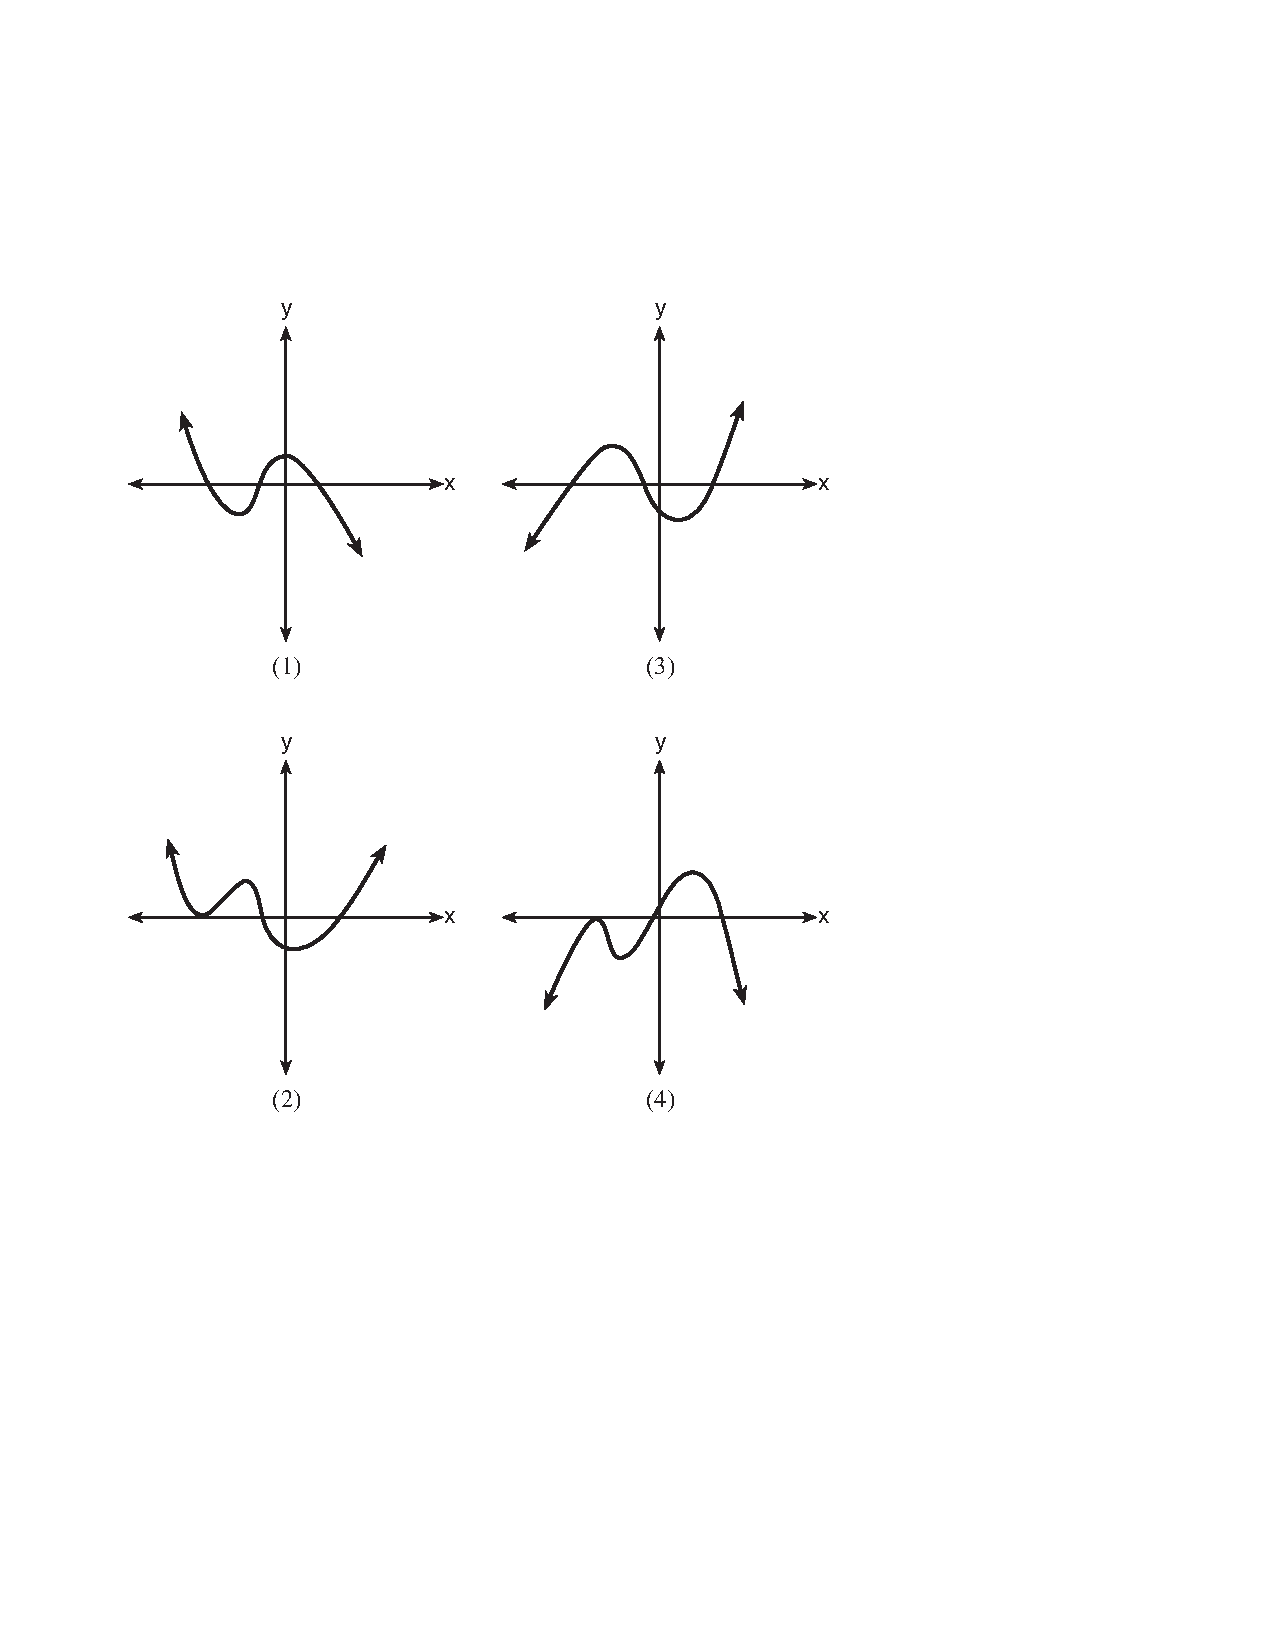
\includegraphics[width=0.75\textwidth]{cubic-graphs.pdf}
\end{figure} %Alg2 Regents Jun2016

\newpage
\item The graph of the function $p(x)$ is sketched below.
\begin{center}
    \begin{tikzpicture}[scale=2.54/4]
    \draw[thick,<->] (-4.5,0) -- (5.5,0) node[anchor=north west] {\textbf{x}};
    \draw[thick,<->] (0,-3.5) -- (0,7.5) node[anchor=south east] {\textbf{p(x)}};
    \foreach \x in {-1, 1} \draw (\x cm,5pt) -- (\x cm,-5pt) node[anchor=north] {$\x$};
    \foreach \x in {-4,-3,-2, 2, 3, 4} \draw (\x cm,5pt) -- (\x cm,-5pt) node[anchor=north] {};
    %\foreach \y in {5} \draw (1pt,\y cm) -- (-1pt,\y cm) node[anchor=east] {50}; %{$\y$};
    \tkzInit[xmin=-5,xmax=5,ymin=-3,ymax=7,ystep=1]   
    \tkzFct[color=black,very thick,<->,domain = -3.2:4] {0.2*(x*x-9)*(x-2)};
    \end{tikzpicture}
\end{center}
Which equation could represent $p(x)$?
\begin{enumerate}
    \item $p(x)=(x^2- 9)(x-2)$
    \item $p(x)=x^3 -2x^2+ 9x+18$
    \item $p(x)=(x^2+ 9)(x-2)$
    \item $p(x)=x^3 +2x^2- 9x-18$
\end{enumerate} %Alg2 Regents Jun2017 multiple choice

\item When $g(x)$ is divided by $x+4$, the remainder is 0. Given $g(x)= x^4+3x^3-6x^2-6x+8$, which conclusion about $g(x)$ is true?
\begin{enumerate}
    \item $g(4)=0$
    \item $g(-4)=0$
    \item $x-4$ is a factor of $g(x)$.
    \item No conclusion can be made regarding $g(x)$.
\end{enumerate} %Alg2 Regents Jan2017 multiple choice

\item The expression $\displaystyle \left( \frac{m^2}{m^\frac{1}{3}}\right)^{-\frac{1}{2}}$ is equivalent to 
\begin{enumerate}
    \item $-\sqrt[6]{m^5}$
    \item $\displaystyle \frac{1}{\sqrt[6]{m^5}}$
    \item $-m \sqrt[5]{m}$
    \item $\displaystyle \frac{1}{m \sqrt[5]{m}}$
\end{enumerate} %Alg2 Regents Jan2017 multiple choice


\end{enumerate}
\end{document}


\item An equation to represent the value of a car after $t$ months of ownership is $\displaystyle v=32,000(0.81)^{\frac{t}{12}}$. Which statement is \emph{not} correct?
\begin{enumerate}
    \item The car lost approximately 19\% of its value each month.
    \item The car maintained approximately 98\% of its value each month.
    \item The value of the car when it was purchased was \$32,000.
    \item The value of the car 1 year after it was purchased was \$25,920.
\end{enumerate} %Alg2 Regents Aug2016 MC
